\subsection{Боксплот Тьюки}
\begin{itemize}
	\item{Нормальное распределение}
	\begin{figure}[H]
		\begin{center}
			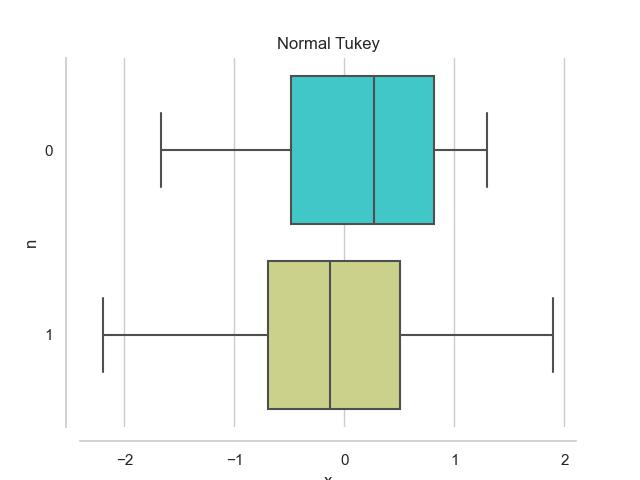
\includegraphics[scale=0.75]{task_3/resource/Normal Tukey.jpg}
			\caption{Нормальное распределение} 
		\end{center}
	\end{figure}
	
	\item{Распределение Коши}
	\begin{figure}[H]
		\begin{center}
			\includegraphics[scale=0.75]{task_3/resource/cauchy Tukey.jpg}
			\caption{Распределение Коши}
		\end{center}
	\end{figure}
		
	\item{Распределение Пуассона}
	\begin{figure}[H]
		\begin{center}
			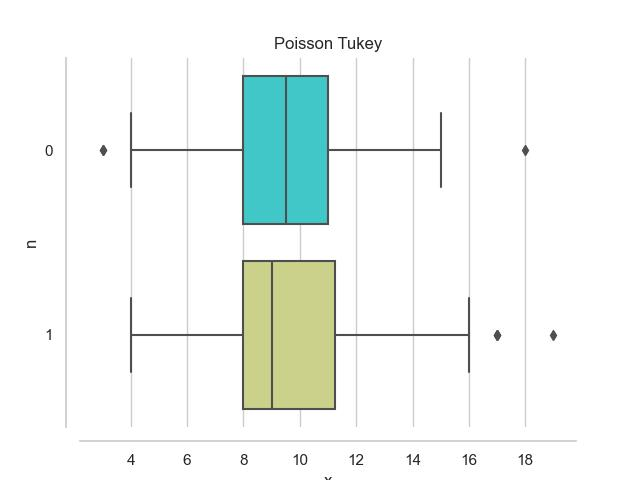
\includegraphics[scale=0.75]{task_3/resource/Poisson Tukey.jpg}
			\caption{Распределение Пуассона} 
		\end{center}
	\end{figure}
	
	\item{Равномерное распределение}
	\begin{figure}[H]
		\begin{center}
			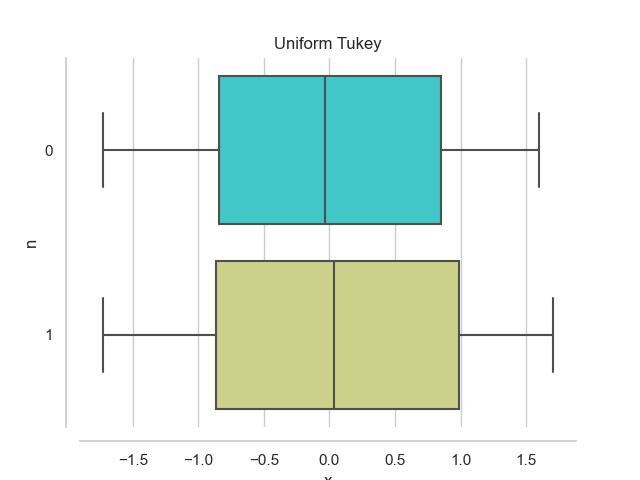
\includegraphics[scale=0.75]{task_3/resource/Uniform Tukey.jpg}
			\caption{Равномерное распределениеы} 
		\end{center}
	\end{figure}

\end{itemize}

\subsection{Доля выбросов}
Выборка случайна, поэтому в качестве оценки рассеяния можно взять дисперсию пуассоновского потока: $D_n \approx \sqrt{n}$ \newline
Доля $p_n = D_n / n = 1 / \sqrt{n}$ \newline
Доля $n = 20$: $p_n = 1 / \sqrt{20}$ - примерно 0.2 или 20\%\proc \newline
Доля $n = 100$: $p_n = 1 / 10$ - 0.1 или 10\% \newline
Из этого можно решить, сколько знаков оставлять в доле выбросов. \newline

\begin{table}[H]
	\centering
		\begin{tabular}[t]{|l|r|}
			\hline
			Выборка & Доля выбросов\\
			\hline
			Normal n = 20   &  0.02\\
			\hline
			Normal n = 100   &  0.02\\
			\hline
			Cauchy n = 20   &  0.15\\
			\hline
			Cauchy n = 100   &  0.18\\
			\hline
			Poisson n = 20   &  0.02 \\
			\hline
			Poisson n = 100   &  0.01 \\
			\hline
			Uniform n = 20   &  0\\
			\hline
			Uniform n = 100   &  0\\
			\hline
		\end{tabular}
		\caption{Доля выбросов}
		\label{tab:normal}
	\end{table}
	
\subsection{Теоретическая вероятность выбросов}
    \begin{table}[H]
	    \centering
		\begin{tabular}[t]{|l|r|r|r|r|r|}
			\hline
			Распределение   &      $Q_1^T$	& $Q_3^T$ & $X_1^T$ & $X_2^T$ & $P_B^T$	\\
			\hline
			Нормальное распределение 	& -0.674& 0.674 & -2.698 	&  2.698 	& 0.007 \\
			\hline
			Распределение Коши 			& -1	& 1		&  -4		& 4			& 0.156 \\
			\hline
			Распределение Пуассона 		& 8		& 12	& 2			& 18		& 0.008 \\
			\hline
			Равномерное распределение 	&-0.866 & 0.866	& -3.464 	& 3.464 	& 0	\\
			\hline
		\end{tabular}
		\caption{Теоретическая вероятность выбросов}
		\label{tab:normal}
\end{table}